\documentclass[a4paper,12pt]{article}

\usepackage[margin=1in]{geometry}
\usepackage{tikz}
\usepackage{amssymb}
\usepackage{xcolor}
\usepackage{circuitikz}
\usepackage{graphicx}

\newcommand{\ra}{$\rightarrow$}
\newenvironment{6mini}{
  \begin{minipage}{6cm}
}{
  \end{minipage}
}

\title{\texttt{Module 3}\\\hrulefill}
\author{\texttt{Logic}}
\date{\small{9/6/2023}}

\begin{document}
    \maketitle

    \section{Binary Codes}
        Binary Code is how information is represented with binary digits, mulitple exist.Codes provide further implementation methods of binary into a digital system.\vspace{5pt}\\
        \textbf{Binary Coded Decimal} is code to represent decimal in binary. Each digit is represented by its binary 4-bit equivalent.\\
        \begin{6mini}
            Application include numeric LED displays. (BCD is translated digit by digit and the appropriate number is shown
            )
        \end{6mini}
        \begin{6mini}
            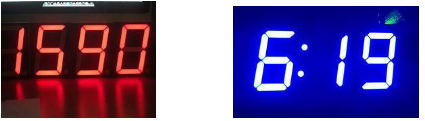
\includegraphics{LED displays.png}
        \end{6mini}
        \section{Logic}
        Logic math (\texttt{Boolean Algebra}) existed before digital computers. It explained logic, by the means of math, utilizing 2 values (\textit{True or False}).
        \begin{itemize}
            \item As a transistor is a binary output, logic can be implemented
            \item Basic functions are \texttt{AND, OR, NOT}
        \end{itemize}
        \hrulefill
        \begin{itemize}
            \item \textbf{AND} \ra All inputs mus tbe true for the expression too be true. $z=xy,z=x~*~y$
           late \item \textbf{OR} \ra Any 1 input can be true for the expression to be true. $z=x+y$
            \item \textbf{NOT} \ra Reverse the expression/scoped output from true to false and vice versa. $z=x'=\bar{x}$
        \end{itemize}
        \begin{center}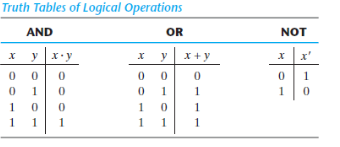
\includegraphics[width=8cm]{Truth Tables.png}\end{center}

    \subsection{Logic gates}
        These functions are implemented with logic gates, Electronic device to implement Boolean function.
        \begin{itemize}
            \item These gatees have mulitple inputs and one output.
            \item They use specific symbols in their schematic representation
        \end{itemize}
        \begin{center}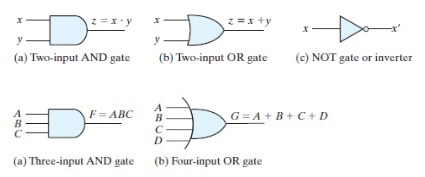
\includegraphics[width=9cm]{Logic Gates.png}\end{center}

    \subsection*{Boolean Functions}
        Varibales are used to represent inputs and outputs. in a Boolean function, ANDs appear as a product and ORs appear as a sum. NOT is represented with a ‘ or a bar above the variable.
        \begin{itemize}
            \item In a Boolean function, ANDs appear as a product and ORs appear as a sum. NOT is represented with a ‘ or a bar above the variable
        \end{itemize}
        \includegraphics*[width=10cm]{circuit1.png}
        \begin{enumerate}
            \item The output of the cicuit, F: 1
            \item Circuit as a boolean expression: $F=\bar{A}B+CD+\bar{E}$
        \end{enumerate}

        \subsection*{Cascading Logic Gates}
            Logic gates can be cascaded together to create more inputs, for physical logic gates only have a finite amount of inputs.

        \subsection*{Timing DIagram}
            SHows inputs and outputs of a logic circuit over time. ouput of a logic circuit is assumed to change "instantly".
            \begin{itemize}
                \item Inputs are on the top, outputs are at the bottom, for the sake of readability.
            \end{itemize}
            \begin{center}\includegraphics*[width=5cm]{Timing Diagram.png}\end{center}

            \subsection*{Truth Tables}
            describes all of the possible input combinations to generate an output. can be developed from observing a schematic, and conversely, a schematic can be developed using a truth table.
            \begin{itemize}
                \item Left hand side \ra inputs from MSB to LSB
                \item Right hand side \ra outputs from MSB to
                \item Number of rows = $2^n$, where n is the number of inputs
            \end{itemize}
            
            \section{Addional logic gates}
                \subsection*{NAND}
                    \[F=(XY)'=NOT(X~and~Y)\]
                    \textbf{Universal Logic gate:} Any gate can be made with NAND
                    \vspace{10pt}\\
                    \includegraphics*[width=10cm]{NAND.png}
                    
                \subsection*{NOR}
                \[F=(X+Y)'=NOT(X~OR~Y)\]
                \includegraphics*[width=10cm]{NOR.png}

                \subsection*{Exclusively OR (XOR)}
                    \[F=X'Y+XY'\textnormal{=x or y but not both}\] \[F=X\oplus  Y\]
                    \includegraphics*[width=15cm]{XOR gate.jpg}
                \subsection*{XNOR}
                    \textbf{*Negated xor gate} \[F=XY+X'Y'\] \includegraphics*[width=15cm]{XNOR gate.jpg}
\end{document}